\documentclass{report}
% Ћирилица: кодирање фонда и језик (српски, ћирилица)
\usepackage[T2A]{fontenc}
\usepackage[utf8]{inputenc}
\usepackage[serbianc]{babel}

% Величина стране и маргине
\usepackage[a4paper,top=2cm,bottom=2cm,left=2.5cm,right=2.5cm]{geometry}

% Корисни пакети
\usepackage{amsmath}
\usepackage{graphicx}
\usepackage{float}
\usepackage{multirow}
\usepackage{array}
\usepackage{enumitem}
\usepackage{tcolorbox}
\tcbuselibrary{skins,breakable}
\usepackage[colorlinks=true, allcolors=blue]{hyperref}

% Главе без нове стране и без великог размака, да се текст лепо пакује
\usepackage{titlesec}
\titleclass{\chapter}{straight}
\titleformat{\chapter}{\normalfont\LARGE\bfseries}{\thechapter.}{0.5em}{}
\titlespacing*{\chapter}{0pt}{18pt}{10pt}

\setcounter{secnumdepth}{2}
\setcounter{tocdepth}{1}

% Мање празнине око слика
\setlength{\textfloatsep}{10pt plus 2pt minus 2pt}
\setlength{\intextsep}{10pt plus 2pt minus 2pt}

% Оквир за кључне податке
\newtcolorbox{kljucno}{breakable, colback=blue!4, colframe=blue!45!black,
    boxrule=0.5pt, arc=1.5pt, left=6pt, right=6pt, top=3pt, bottom=3pt}

% Оквир за поделе: ужи, центриран, наслов на ивици оквира
\newtcolorbox{podela}[1]{enhanced, width=0.85\linewidth, center,
    colback=green!3, colframe=green!45!black, boxrule=0.6pt, arc=2pt,
    title={#1}, fonttitle=\bfseries\small, coltitle=white,
    colbacktitle=green!45!black,
    attach boxed title to top left={xshift=4mm, yshift=-2.2mm},
    boxed title style={boxrule=0pt, arc=1pt},
    top=4mm, bottom=2mm, left=2mm, right=2mm, fontupper=\small,
    before skip=8pt, after skip=8pt}

% Нумерисана листа унутар подела
\newlist{lista}{enumerate}{2}
\setlist[lista,1]{label=\arabic*., noitemsep, topsep=0pt, leftmargin=1.6em}
\setlist[lista,2]{label=\alph*), noitemsep, topsep=0pt, leftmargin=1.4em}

% Већа слика (шеме): до 9 cm висока
\newcommand{\slikaV}[4][0.7]{%
\begin{figure}[!htb]
    \centering
    \IfFileExists{slike/#2}%
        {\includegraphics[width=#1\textwidth,height=9cm,keepaspectratio]{slike/#2}}%
        {\fbox{\parbox[c][4cm][c]{#1\textwidth}{\centering\small слика: \texttt{slike/#2}}}}
    \caption{#3}
    \label{#4}
\end{figure}}

% Слика: мала, највише 5 cm висока, плута да не оставља празна места
\newcommand{\slika}[4][0.45]{%
\begin{figure}[!htb]
    \centering
    \IfFileExists{slike/#2}%
        {\includegraphics[width=#1\textwidth,height=5cm,keepaspectratio]{slike/#2}}%
        {\fbox{\parbox[c][2.5cm][c]{#1\textwidth}{\centering\small слика: \texttt{slike/#2}}}}
    \caption{#3}
    \label{#4}
\end{figure}}

\title{Аутоелектронски системи 2 - M-Motronic}
\author{Саобраћајно техничка школа, Београд, Земун}
\date{}

\begin{document}
\maketitle
\tableofcontents
\newpage

%##################################################################
\chapter{Систем Bosch M-Motronic}
%##################################################################

Систем \textbf{Bosch M-Motronic} обједињује електронско паљење и убризгавање.
Целокупна електроника којом се регулише рад мотора, са свим регулационим и
управљачким функцијама, налази се у електронској (централној) управљачкој
јединици (ECU). Потребни подаци и параметри који карактеришу рад мотора
прикупљају се помоћу више сензора.

\begin{kljucno}
Управљачка јединица прикупља аналогне и дигиталне сигнале са сензора, обрађује
их у микропроцесору и преко излазних степена снаге управља извршним органима
(бризгаљке, бобина, релеји, актуатори), чиме се у свим режимима рада мотора
остварује оптимално убризгавање смеше уз најповољнији тренутак паљења.
\end{kljucno}

Сензори прикупљају податке о систему паљења, положају брегастог и коленастог
вратила, брзини возила, тренутном преносном односу у мењачу, клима-уређају итд.
Посебну групу чине аналогни улазни сигнали: напон акумулатора, температура
ваздуха и мотора, количина усисаног ваздуха, угао пригушног лептира, ЛАМБДА
сонда, детонантнo сагоревање (кликтање мотора) и број обртаја мотора.

\slikaV[0.85]{1.jpg}{}{fig:m_motronic_shema}

\begin{kljucno}
    \begin{enumerate}
    \item регенератор са активним угљем
    \item вентил за ваздух
    \item електрични (EVAP) вентил регенератора
    \item регулатор притиска за гориво
    \item бризгаљка
    \item регулатор притиска у усисној цеви
    \item индукциони калем -- бобина
    \item сензор фазе
    \item пумпа за секундарни ваздух
    \item вентил секундарног ваздуха
    \item мерач протока ваздуха -- протокомер
    \item електронска или централна управљачка јединица (CPU)
    \item давач положаја пригушног лептира
    \item регулатор празног хода
    \item сензор температуре ваздуха
    \item вентил за повраћај (рециркулацију) издувних гасова
    \item филтер за гориво
    \item сензор кликтања
    \item сензор броја обртаја мотора
    \item сензор температуре мотора
    \item ЛАМБДА сонда
    \item прикључак за дијагностику
    \item сигнална лампица прикључка
    \item сензор разлике притиска
    \item резервоар за гориво са уграђеном електричном пумпом
\end{enumerate}
\end{kljucno}

\begin{podela}{Функције M-Motronic система}
\begin{lista}
    \item \textbf{Основне функције:}
    \begin{lista}
        \item управљање паљењем и убризгавањем горива,
        \item прикупљање и обрада основних параметара о раду мотора и мерних величина.
    \end{lista}
    \item \textbf{Додатне функције:}
    \begin{lista}
        \item регулација броја обртаја у празном ходу,
        \item ЛАМБДА регулација састава смеше,
        \item регенерација испареног горива из резервоара,
        \item рециркулација (повраћај) издувних гасова ради смањења емисије $\text{NO}_x$,
        \item управљање радом турбо-пуњача ради повећања снаге мотора,
        \item подешавање брегастог вратила (фазни дијаграм вентила),
        \item заштита од детонантнoг сагоревања (кликтања мотора),
        \item ограничење прекорачења броја обртаја мотора и брзине кретања возила.
    \end{lista}
\end{lista}
\end{podela}

\paragraph*{Електронски системи управљања (Менаџмент мотора).}
Повезивањем централне управљачке јединице са управљачким јединицама других
система, M-MOTRONIC потпомаже и усклађује њихов рад. На пример, повезивање са
управљачком јединицом аутоматског мењача омогућава смањење потиска током
преноса (штити механизам мењача и повећава удобност вожње), док заједно са
ABS и ASR системима повећава стабилност вожње.

%==================================================================
\section{Инсталација за напајање горивом}
%==================================================================

Задатак инсталације за напајање горивом је да у свим режимима рада мотору
обезбеди довољну количину горива. Електрична пумпа преко филтера потискује
гориво из резервоара ка главној разводној цеви (разделнику) на којој се
налазе бризгаљке и регулатор притиска (слика~\ref{fig:napajanje_gorivom}).

\slika[0.65]{2.jpg}{Инсталација за напајање горивом: 1. електрична пумпа у резервоару, 2. филтер за гориво, 3. главна разводна цев, 4. бризгаљка, 5. регулатор притиска}{fig:napajanje_gorivom}

Бризгаљке убризгавају гориво у простор испред усисних вентила у усисним гранама,
а регулатор одржава константан притисак у разводној цеви. Вишак горива се
преко регулатора враћа у резервоар, чиме се гориво хлади и спречава стварање
ваздушних мехурића. На бризгаљкама се одржава разлика притиска од око
\textbf{300~kPa (3~bar)}. По потреби се уграђује и хидраулична пригушница
(шпајхер) за ублажавање осцилација притиска.

\subsection{Електрична пумпа за гориво}

Електрична пумпа се најчешће поставља у резервоар заједно са показивачем нивоа
горива и посудом за одвајање ваздушних мехурића из повратног вода. Ако се
постави у напојни вод, постоји опасност да повуче ваздух, па се у резервоар
додаје помоћна пумпа ниског притиска.

\begin{podela}{Подела пумпи за гориво према конструкцији}
\begin{lista}
    \item \textbf{Потисне пумпе:}
    \begin{lista}
        \item ваљчасте пумпе са ћелијама (остварују притисак до 6~bar),
        \item зупчасте пумпе са унутрашњим озубљењем (притисак до 4~bar).
    \end{lista}
    \item \textbf{Хидрауличне (центрифугалне) пумпе:}
    \begin{lista}
        \item са периферним каналима и лопатицама (притисак до 3~bar, без пулсирања и буке),
        \item са бочним каналима и двоструким радним колом (притисак око 1~bar -- за централно убризгавање или као предстепен).
    \end{lista}
\end{lista}
\end{podela}

\slikaV[0.75]{3.jpg}{Принцип рада потисних и хидрауличних пумпи: а) ваљчаста пумпа са ћелијама, б) центрифугална пумпа са периферним каналима и лопатицама, в) зупчаста пумпа са унутрашњим озубљењем, г) центрифугална пумпа са бочним каналима и лопатицама}{fig:pumpe}

\begin{itemize}[noitemsep]
    \item \textbf{Ваљчасте пумпе} имају радно коло са ваљцима који се услед
          центрифугалне силе приљубљују уз ексцентрично кућиште и формирају
          коморе променљиве запремине (слика~\ref{fig:pumpe}а).
    \item \textbf{Зупчасте пумпе} имају мањи погонски зупчаник унутар већег
          ексцентрично постављеног зупчаника са једним зубом више (слика~\ref{fig:pumpe}в).
    \item \textbf{Центрифугалне пумпе} убрзавају честице течности помоћу лопатица
          радног кола и потискују их ка излазном каналу (слике~\ref{fig:pumpe}б и \ref{fig:pumpe}г).
\end{itemize}

\subsection{Филтер за гориво и главна разводна цев}

\textbf{Филтер за гориво} је неопходан ради заштите бризгаљки и регулатора
притиска од нечистоћа. Користе се уобичајени папирни, микропорозни филтери.

\textbf{Главна разводна цев (разделник)} равномерно напаја горивом све бризгаљке.
Конструисана је тако да онемогућава локалну промену притиска услед брзог
укључивања бризгаљки. На њу се постављају бризгаљке, регулатор притиска и по
потреби хидраулична пригушница. Израђује се од челичног лима, алуминијума или
специјалних синтетичких материјала.

\subsection{Регулатор притиска и хидраулична пригушница}

\textbf{Регулатор притиска} одржава константан пад притиска на бризгаљкама,
како би количина убризганог горива зависила искључиво од времена отварања
бризгаљке. Ради на принципу мембранског преливног вентила :
када притисак горива порасте изнад подешене вредности, еластична мембрана
савлада силу опруге, отвори вентил и вишак горива врати у резервоар. Горња
комора са опругом спојена је са усисном цеви иза пригушног лептира, па је
разлика притиска на бризгаљкама увек константна.

\textbf{Хидраулична пригушница (шпајхер)} умирује периодичне осцилације притиска
које потичу од пулсирања електричне пумпе и рада бризгаљки. Изнад еластичне
мембране налази се ваздушна комора са опругом, а испод гориво под притиском;
променом запремине доње коморе пригушују се осцилације.


%==================================================================
\section{Убризгавање горива}
%==================================================================

Убризгана количина горива мора бити сразмерна количини усисаног ваздуха.
Сваком цилиндру припада електромагнетна бризгаљка која гориво убризгава
непосредно испред усисног вентила, чиме се избегава кондензација горива на
зидовима усисне цеви и поремећај коефицијента вишка ваздуха ($\lambda$).

\subsection{Електромагнетна бризгаљка}

Иглица бризгаљке под дејством електромагнета подиже се за свега \textbf{60--100~$\mu$m}.
Кроз калибрисани отвор гориво се испушта за \textbf{1,5--18~ms}, са учестаношћу
од \textbf{3--125~Hz} (зависно од броја обртаја мотора).

\begin{podela}{Типови електромагнетних бризгаљки}
\begin{lista}
    \item \textbf{Бризгаљка са горњим уливом (top-feed):} гориво улази с горње
          стране и аксијално струји кроз седиште бризгаљке; причвршћује се
          заптивним прстеновима за разводну и усисну цев.
    \item \textbf{Бризгаљка са бочним уливом (bottom-feed):} уграђује се директно
          у главну разводну цев, гориво улази бочно и протиче по целом обиму
          бризгаљке; обезбеђује мању висину модула и боље хлађење горива.
\end{lista}
\end{podela}

\slika[0.75]{3.1.jpg}{Главна разводна цев са уграђеним бризгаљкама са бочним уливом: 1. улаз горива, 2. бризгаљка, 3. електрични прикључак, 4. контактне траке, 5. регулатор притиска, 6. излаз горива}{fig:razvodna_cev}

\subsection{Начин убризгавања горива и облици млазница}

Ради што бољег распршивања и хомогенизацие горива и ваздуха израђују се
различите млазнице (слика~\ref{fig:mlaznice}):
\begin{itemize}[noitemsep]
    \item \textbf{Прстенаста млазница} -- образује је врх иглице и отвор седишта вентила.
    \item \textbf{Млазница са једном рупицом} -- даје танак, оштар млаз који не кваси зидове усисне цеви.
    \item \textbf{Млазница са више рупица} -- даје шири млаз и може формирати дводелне млазове (погодно за моторе са више усисних вентила по цилиндру).
    \item \textbf{Бризгаљка са ваздушним испирањем} -- део усисаног ваздуха пролази кроз саму бризгаљку великом брзином и даје најфиније распршивање.
\end{itemize}

\begin{figure}[!htb]
    \centering
    \begin{minipage}{0.48\textwidth}
        \centering
        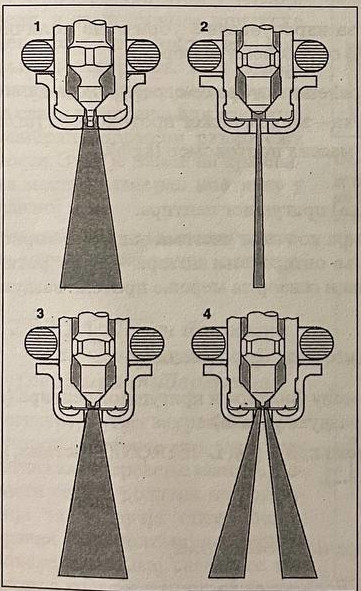
\includegraphics[height=5.2cm,keepaspectratio]{slike/4.jpg}
        \caption{Начин убризгавања горива млазницама различитог облика: 1. прстенаста, 2. са једном рупицом, 3. са више рупица, 4. са више рупица и два млаза}
        \label{fig:mlaznice}
    \end{minipage}\hfill
\end{figure}

%==================================================================
\section{Прикупљање података о раду мотора (Сензори)}
%==================================================================

\subsection{Оптерећење мотора и мерење протока ваздуха}

Оптерећење мотора један је од најважнијих података за израчунавање количине
горива и угла паљења. Одређује се помоћу:
\begin{itemize}[noitemsep]
    \item \textbf{Запреминског протокомера} ($\text{m}^3/\text{h}$) -- поставља се између филтера и пригушног лептира и мери угао отклањања мерне плоче (клапне) под дејством струје ваздуха (слика~\ref{fig:zapreminski_protokomer}).
    \item \textbf{Масеног протокомера} ($\text{kg/h}$) -- користи термичке сензоре са \textbf{ужареним влакном} или \textbf{врелим филмом} (платински отпорник на керамичкој плочици). Електроника одржава сталну температурну разлику грејног елемента у односу на ваздух, па је струја грејања директна мера масеног протока и густине ваздуха (слике~\ref{fig:vreli_film_kuciste} и \ref{fig:vreli_film_sema}).
    \item \textbf{Сензора притиска у усисном воду (MAP)} -- пиезо-отпорници у мостној вези на дебелослојној мембрани мере апсолутни притисак у усисној цеви (слика~\ref{fig:map_senzor}).
    \item \textbf{Давача положаја пригушног лептира (TPS)} -- потенциометар на осовини лептира региструје угао отварања за празан ход, делимично и пуно оптерећење (слика~\ref{fig:tps_senzor}).
\end{itemize}

\slika[0.7]{5.jpg}{Запремински протокомер: 1. пригушни лептир, 2. протокомер, 3. сигнал температуре ваздуха, 4. електронска управљачка јединица, 5. сигнал мерача протока ваздуха, 6. филтер за ваздух}{fig:zapreminski_protokomer}

\begin{figure}[!htb]
    \centering
    \begin{minipage}{0.48\textwidth}
        \centering
        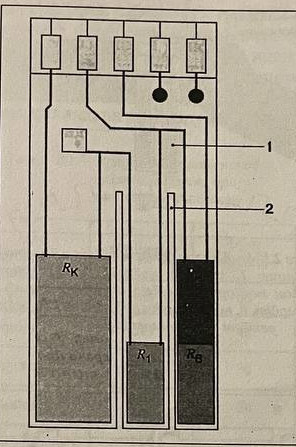
\includegraphics[height=5cm,keepaspectratio]{slike/6.0.jpg}
        \caption{Мерач протока ваздуха са врелим филмом: а) кућиште, б) сензор са врелим филмом (1. ребра за хлађење, 2. преносни елемент, 3. излазни елемент, 4. хибридна веза, 5. плочица сензора)}
        \label{fig:vreli_film_kuciste}
    \end{minipage}\hfill
    \begin{minipage}{0.48\textwidth}
        \centering
        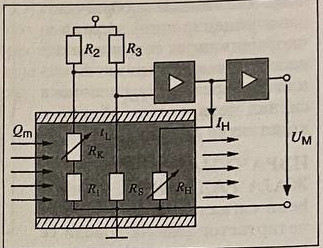
\includegraphics[height=5cm,keepaspectratio]{slike/6.1.jpg}
        \caption{Шема везе протокомера са врелим филмом: $R_K$ -- температурна компензација, $R_H$ -- загревни отпорник, $R_1, R_2, R_3$ -- отпорници у мостној вези, $U_M$ -- излазни напон}
        \label{fig:vreli_film_sema}
    \end{minipage}
\end{figure}

\begin{figure}[!htb]
    \centering
    \begin{minipage}{0.48\textwidth}
        \centering
        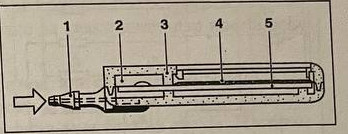
\includegraphics[height=4.8cm,keepaspectratio]{slike/7.0.jpg}
        \caption{Сензор притиска у усисном воду: 1. прикључак за црево, 2. ћелија под притиском, 3. преграда са заптивком, 4. електронска веза, 5. дебелослојни хибрид}
        \label{fig:map_senzor}
    \end{minipage}\hfill
    \begin{minipage}{0.48\textwidth}
        \centering
        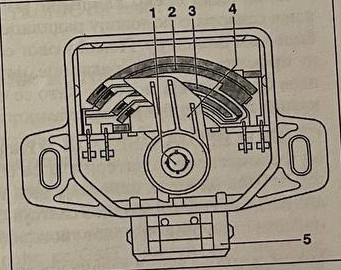
\includegraphics[height=4.8cm,keepaspectratio]{slike/7.1.jpg}
        \caption{Давач положаја пригушног лептира: 1. осовина лептира, 2. отпорно поље са једноструким сигналом, 3. отпорно поље са двоструким сигналом, 4. клизач са контактима, 5. електрични прикључак}
        \label{fig:tps_senzor}
    \end{minipage}
\end{figure}

\subsection{Број обртаја мотора и положај радилице и брегастог вратила}

\textbf{Сензор броја обртаја и положаја радилице (индуктивни давач):} на радилицу се
поставља феромагнетни зупчасти точак са \textbf{60 зубаца од којих недостају два}.
Изнад њега је индуктивни сензор са сталним магнетом и намотајем (слика~\ref{fig:senzor_radilice}).
Пролазак зубаца индукује наизменични напон чија учестаност даје број обртаја,
док шупљина од два недостајућа зуба служи као референтни знак положаја радилице
у односу на први цилиндар. Сваки импулс одговара углу од $3^\circ$, а дељењем на
четири дела добија се резолуција од $0,75^\circ$ за прецизно одређивање угла паљења.

\textbf{Положај брегастог вратила (Холов давач):} брегасто вратило се окреће упола
спорије од радилице и одређује да ли је клип у такту сабијања или издувавања
(неопходно за секвенцијално убризгавање и статичко паљење). Најчешће се користи
\textbf{Холов давач} који при проласку феромагнетне бленде генерише четвртасти
напонски сигнал (слика~\ref{fig:signali_radilica_bregasta}).

\begin{figure}[!htb]
    \centering
    \begin{minipage}{0.46\textwidth}
        \centering
        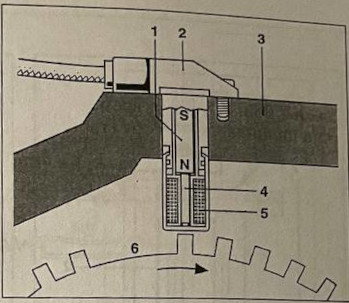
\includegraphics[height=4.8cm,keepaspectratio]{slike/8.1.jpg}
        \caption{Сензор броја обртаја и положаја радилице: 1. стални магнет, 2. поклопац, 3. блок мотора, 4. језгро од меког гвожђа, 5. намотај, 6. недостајући зуб (референтни знак)}
        \label{fig:senzor_radilice}
    \end{minipage}\hfill
    \begin{minipage}{0.50\textwidth}
        \centering
        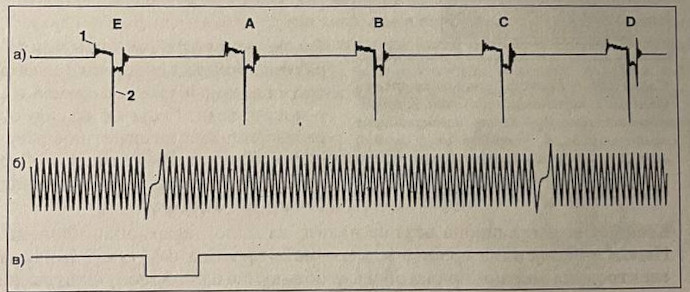
\includegraphics[height=4.8cm,keepaspectratio]{slike/8.0.jpg}
        \caption{Зависност тренутка паљења од положаја радилице и брегасте осовине: а) секундарни напон бобине, б) сигнали сензора радилице, в) сигнали Холовог сензора}
        \label{fig:signali_radilica_bregasta}
    \end{minipage}
\end{figure}

Код четворотактних мотора радилица се окрене за $720^\circ$ током једног радног
циклуса, па просечан угаони размак паљења (\emph{временски сегмент}) зависи од
броја цилиндара (табела~\ref{tab:vremenski_segment}).

\begin{table}[!htb]
    \centering
    \small
    \begin{tabular}{|l|c|c|c|c|c|c|c|}
        \hline
        \textbf{Број цилиндара} & 2 & 3 & 4 & 5 & 6 & 8 & 12 \\ \hline
        \textbf{Степени радилице} & $360^\circ$ & $240^\circ$ & $180^\circ$ & $144^\circ$ & $120^\circ$ & $90^\circ$ & $60^\circ$ \\ \hline
        \textbf{Број зубаца (од 60)} & 60 & 40 & 30 & 24 & 20 & 15 & 10 \\ \hline
    \end{tabular}
    \caption{Вредности временског сегмента према броју цилиндара у мотору}
    \label{tab:vremenski_segment}
\end{table}

\subsection{Остали сензори система}

\begin{itemize}[noitemsep]
    \item \textbf{Ламбда сонда} -- уграђује се у издувни систем и мери садржај кисеоника ради одржавања стехиометријског односа смеше ($\lambda = 1$).
    \item \textbf{Сензор кликтања (детонације)} -- пиезо-керамички сензор на блоку мотора (1 код четвороцилиндричних, 2 или више код вишецилиндричних мотора) који карактеристичне механичке вибрације при детонантном сагоревању претвара у електрични сигнал (слике~\ref{fig:senzor_kliktanja} и \ref{fig:mesta_kliktanja}).
    \item \textbf{Сензори температуре мотора и усисаног ваздуха} -- NTC отпорници за корекцију смеше при хладном старту и промени густине ваздуха.
    \item \textbf{Напон акумулатора} -- прати се ради компензације кашњења отварања електромагнета бризгаљке при паду напона.
\end{itemize}

\begin{figure}[!htb]
    \centering
    \begin{minipage}{0.48\textwidth}
        \centering
        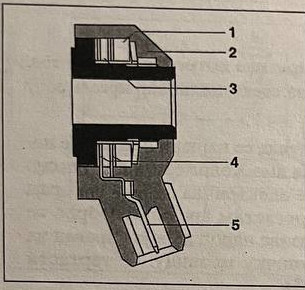
\includegraphics[height=4.8cm,keepaspectratio]{slike/10.0.jpg}
        \caption{Сензор кликтања: 1. сеизмички материјал, 2. маса за заливање, 3. пиезо-керамика, 4. контакти, 5. електрични прикључак}
        \label{fig:senzor_kliktanja}
    \end{minipage}\hfill
    \begin{minipage}{0.48\textwidth}
        \centering
        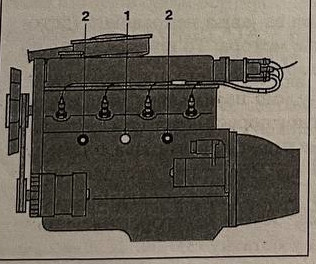
\includegraphics[height=4.8cm,keepaspectratio]{slike/10.1.jpg}
        \caption{„Прислушна” места сензора кликтања на блоку мотора: 1. за четвороцилиндрични мотор, 2. за шестоцилиндрични мотор}
        \label{fig:mesta_kliktanja}
    \end{minipage}
\end{figure}

%==================================================================
\section{Обрада података, време и начин убризгавања}
%==================================================================

\subsection{Време убризгавања}

\textbf{Основно време убризгавања} израчунава се из оптерећења мотора и константе
бризгаљке за идеалан стехиометријски састав смеше ($\lambda = 1$).
\textbf{Ефективно (стварно) време убризгавања} добија се након низа корекција:
након старта и при загревању, корекције ЛАМБДА регулације, искључења при кочењу
мотором, прелазних компензација (убрзање/успоравање), корекције оптерећења и
корекције напона акумулатора (слика~\ref{fig:vreme_ubrizgavanja}).

\subsection{Начин и положај убризгавања}

\begin{podela}{Начини убризгавања горива}
\begin{lista}
    \item \textbf{Симултано убризгавање:} све бризгаљке убризгавају истовремено --
          једном по сваком обртају радилице, тј. два пута по радном циклусу (слика~\ref{fig:nacin_ubrizgavanja}а).
    \item \textbf{Групно убризгавање:} бризгаљке су подељене у две групе, при чему
          свака група убризгава једном по радном циклусу ($720^\circ$), чиме се
          избегава убризгавање у отворен усисни вентил (слика~\ref{fig:nacin_ubrizgavanja}б).
    \item \textbf{Секвенцијално убризгавање:} свака бризгаљка убризгава појединачно,
          у оптималном тренутку према реду паљења за сваки цилиндар (слика~\ref{fig:nacin_ubrizgavanja}в).
\end{lista}
\end{podela}

\begin{figure}[!htb]
    \centering
    \begin{minipage}{0.48\textwidth}
        \centering
        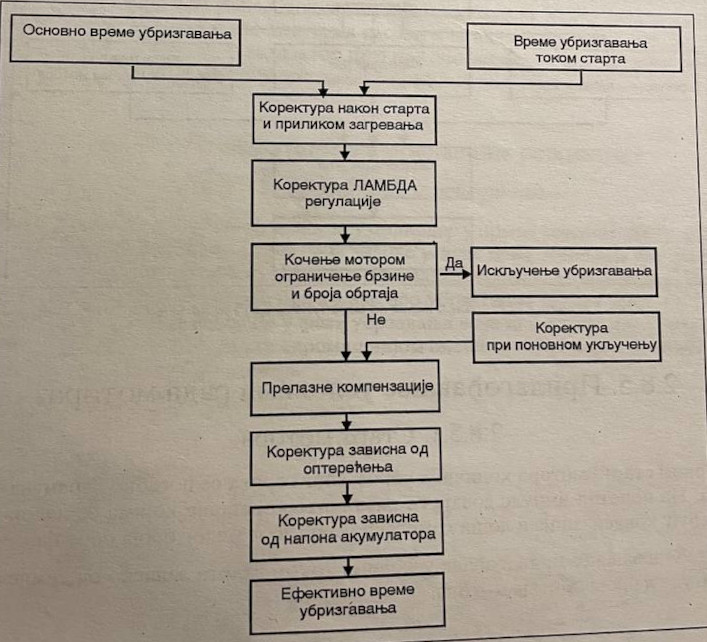
\includegraphics[height=6.2cm,keepaspectratio]{slike/11.1.jpg}
        \caption{Блок шема израчунавања ефективног времена убризгавања}
        \label{fig:vreme_ubrizgavanja}
    \end{minipage}\hfill
    \begin{minipage}{0.48\textwidth}
        \centering
        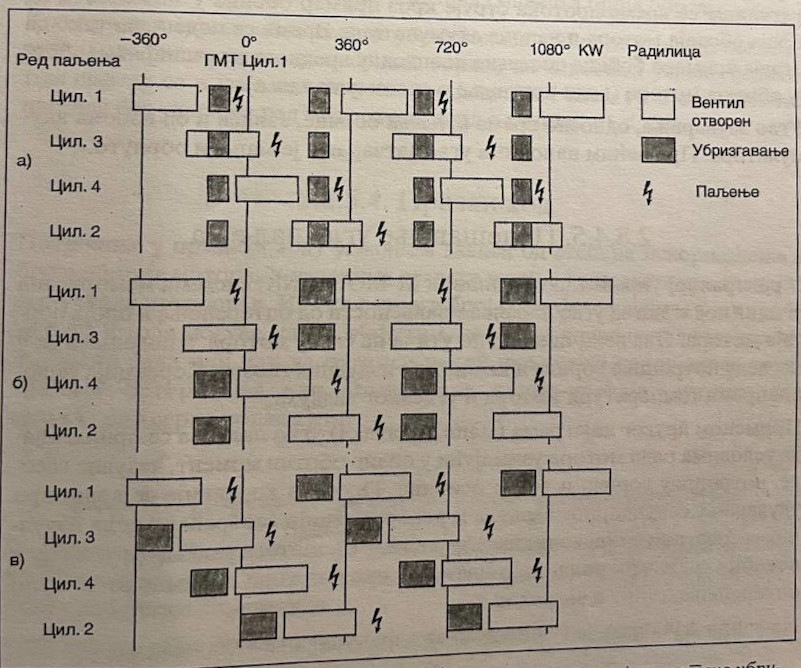
\includegraphics[height=6.2cm,keepaspectratio]{slike/11.jpg}
        \caption{Упоређење начина убризгавања: а) симултано, б) груписано, в) секвенцијално убризгавање}
        \label{fig:nacin_ubrizgavanja}
    \end{minipage}
\end{figure}

\subsection{Угао затварања и угао паљења}

\textbf{Угао затварања (примарне струје)} одређује време пуњења бобине према
тродимензионалној мапи у зависности од броја обртаја и напона акумулатора
(при вишем напону угао затварања је мањи, и обрнуто).

\textbf{Угао паљења} чита се из основне мапе података (оптерећење и број обртаја),
а затим коригује према температури мотора и ваздуха, режиму старта и загревања,
кочењу мотором, регулацији празног хода и регулацији кликтања мотора
(слика~\ref{fig:ugao_paljenja}).

%==================================================================
\section{Прилагођавање условима рада мотора и регулације}
%==================================================================

\begin{itemize}
    \item \textbf{Старт и загревање мотора:} при старту се количина горива
          посебно израчунава ради компензације кондензације на хладним зидовима.
          Током загревања користи се обогаћена смеша уз удувавање секундарног
          ваздуха у издувни систем ради бржег загревања катализатора.
    \item \textbf{Прелазни режими и кочење мотором:} при наглом убрзању додаје се
          гориво због стварања течног филма у усисној цеви, а при успоравању се
          смањује (слика~\ref{fig:prelazni_rezimi}). При кочењу мотором (пуштен гас,
          обртаји изнад празног хода) убризгавање се потпуно искључује ради уштеде
          горива и смањења емисије.
    \item \textbf{Регулација празног хода:} одржава стабилан број обртаја у празном
          ходу при укључивању потрошача (клима, серво, електрична оптерећења)
          помоћу обилазног вода (bypass) или степ-мотора на пригушном лептиру,
          уз брзу фину корекцију променом угла паљења (слика~\ref{fig:prazan_hod}).
\end{itemize}

\begin{figure}[!htb]
    \centering
    \begin{minipage}{0.48\textwidth}
        \centering
        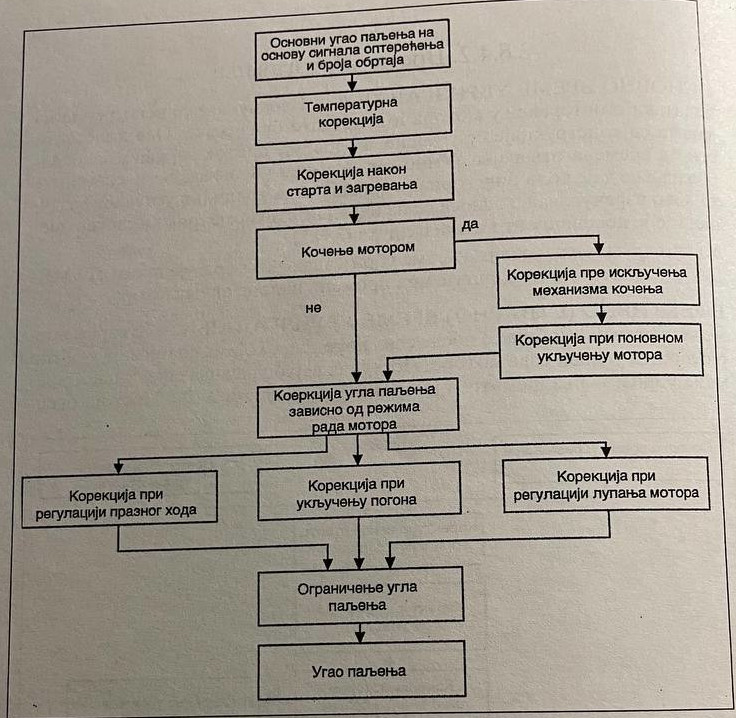
\includegraphics[height=5.5cm,keepaspectratio]{slike/12.1.jpg}
        \caption{Блок шема за израчунавање угла паљења}
        \label{fig:ugao_paljenja}
    \end{minipage}\hfill
    \begin{minipage}{0.48\textwidth}
        \centering
        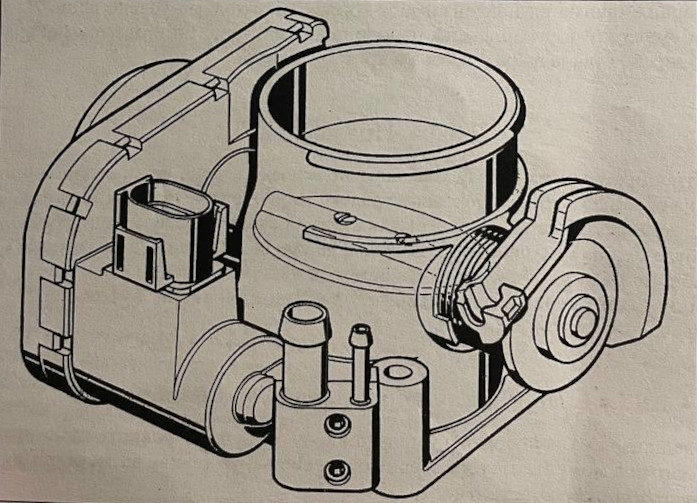
\includegraphics[height=5.5cm,keepaspectratio]{slike/12.2.jpg}
        \caption{Подешавање почетног положаја пригушног лептира помоћу степ-мотора}
        \label{fig:prazan_hod}
    \end{minipage}
\end{figure}

\subsection{Ламбда регулација и регулација са две сонде}

Тростепени катализатор ефикасно претвара $\text{CO}$, $\text{CH}$ и $\text{NO}_x$
само у уском \textbf{ЛАМБДА прозору} ($\lambda = 0,99\dots1,00$). Сонда испред
катализатора на радној температури изнад $350^\circ\text{C}$ даје напон око
\textbf{100~mV} за сиромашну смешу ($\lambda > 1$) и око \textbf{800~mV} за богату
смешу ($\lambda < 1$), са оштрим скоком при $\lambda = 1$ (слика~\ref{fig:lambda_prozor}).

Код савремених система уграђује се и \textbf{друга ламбда сонда иза катализатора}
(слика~\ref{fig:lambda_dve_sonde}), која је заштићенија од високих температура,
компензује старење прве сонде и омогућава дијагностику исправности катализатора.

\begin{figure}[!htb]
    \centering
    \begin{minipage}{0.48\textwidth}
        \centering
        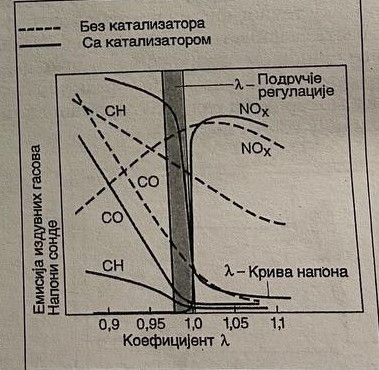
\includegraphics[height=5.2cm,keepaspectratio]{slike/13.1.jpg}
        \caption{Подручје регулације ЛАМБДА сонде и смањење емисије штетних материја}
        \label{fig:lambda_prozor}
    \end{minipage}\hfill
    \begin{minipage}{0.48\textwidth}
        \centering
        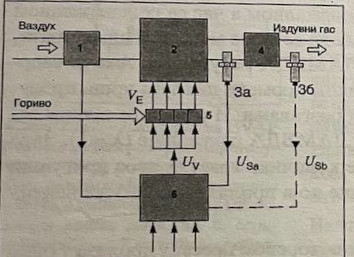
\includegraphics[height=5.2cm,keepaspectratio]{slike/13.2.jpg}
        \caption{Шематски приказ рада ЛАМБДА регулације са две сонде: 1. протокомер, 2. мотор, 3а. прва сонда, 3б. друга сонда, 4. катализатор, 5. бризгаљка, 6. ECU}
        \label{fig:lambda_dve_sonde}
    \end{minipage}
\end{figure}

\subsection{Регенерација испареног горива (EVAP) и заштита од кликтања}

\textbf{Регенерација испареног горива (EVAP):} бензинске паре из резервоара
апсорбују се у посуди са активним угљем (\emph{регенератору}). Током рада мотора
отвара се електрични \textbf{EVAP вентил}, па потпритисак у усисној цеви усисава
свеж ваздух кроз активни угаљ и одводи паре горива на сагоревање (слика~\ref{fig:evap}).

\textbf{Регулација кликтања и притиска турбо-пуњача:} када сензор кликтања
детектује детонацију у неком цилиндру, ECU тренутно помера угао паљења тог
цилиндра ка каснијем, а по престанку кликтања постепено га враћа ка ранијем
(слика~\ref{fig:kliktanje_algoritam}). Код турбо-мотора, ако померање угла паљења
није довољно, ECU помоћу тактног вентила и обилазног вентила (\emph{waste-gate})
снижава притисак пуњења турбо-пуњача (слика~\ref{fig:turbo_regulacija}).

\begin{figure}[!htb]
    \centering
    \begin{minipage}{0.48\textwidth}
        \centering
        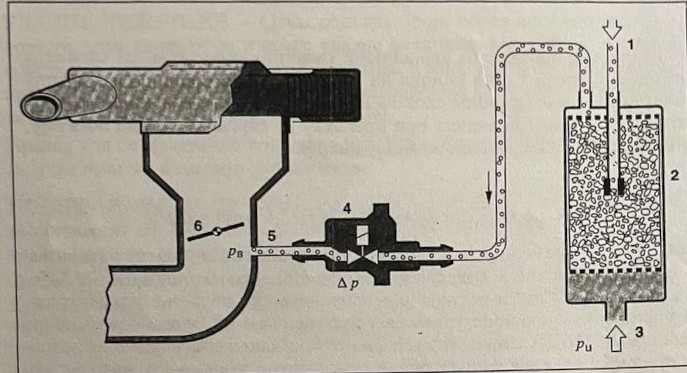
\includegraphics[height=5.2cm,keepaspectratio]{slike/14.1.jpg}
        \caption{Уређај за регенерацију испареног горива: 1. одушак резервоара, 2. регенератор са активним угљем, 3. улаз свежег ваздуха, 4. EVAP вентил, 5. спој на усисну цев, 6. пригушни лептир}
        \label{fig:evap}
    \end{minipage}\hfill
    \begin{minipage}{0.48\textwidth}
        \centering
        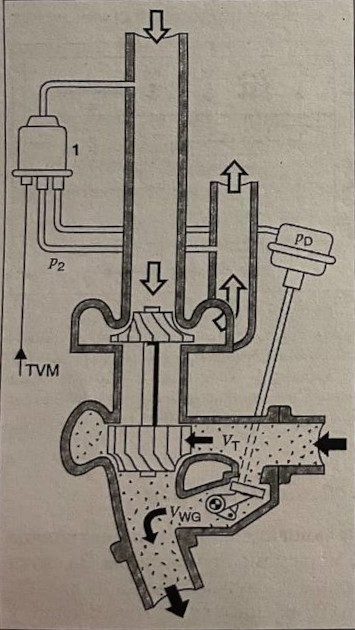
\includegraphics[height=5.2cm,keepaspectratio]{slike/14.2.jpg}
        \caption{Механизам електронске регулације притиска турбо-пуњача: 1. тактни вентил, $p_2$ -- турбопритисак, $p_D$ -- притисак у мембранској ћелији, $TVM$ -- управљачки сигнал}
        \label{fig:turbo_regulacija}
    \end{minipage}
\end{figure}

\subsection{Рециркулација издувних гасова (EGR), подешавање брегастог вратила и усисног вода}

\begin{itemize}[noitemsep]
    \item \textbf{Рециркулација издувних гасова (EGR):} враћањем дела издувних гасова
          у усисну цев снижава се максимална температура сагоревања и смањује
          стварање азотних оксида ($\text{NO}_x$) (слика~\ref{fig:egr}).
    \item \textbf{Подешавање брегастог вратила (VVT):} закретањем брегастог вратила
          или прекопчавањем брегова мењају се фазе отварања и затварања вентила ради
          већег обртног момента, мирнијег празног хода и мање потрошње (слика~\ref{fig:bregasta}).
    \item \textbf{Прекопчавање усисног вода:} коришћењем дужих усисних цеви при малим
          обртајима и краћих при великим обртајима (помоћу клапни и резонантних
          комора) повећава се пуњење цилиндара у целом опсегу обртаја (слика~\ref{fig:usisni_vod}).
\end{itemize}

\begin{figure}[!htb]
    \centering
    \begin{minipage}{0.48\textwidth}
        \centering
        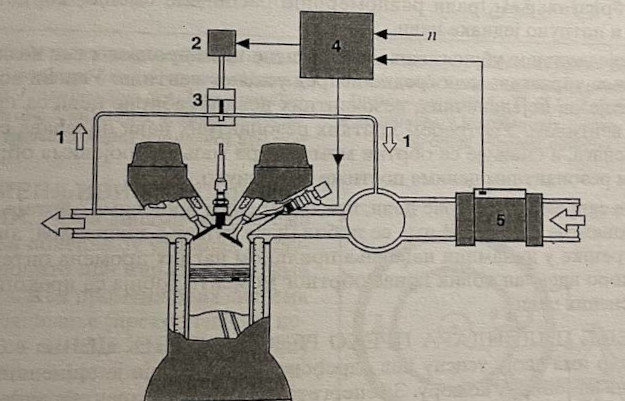
\includegraphics[height=4.8cm,keepaspectratio]{slike/15.1.jpg}
        \caption{Електронско подешавање рециркулације издувних гасова (EGR): 1. повратни вод, 2. електропнеуматски регулатор, 3. вентил рециркулације, 4. ECU, 5. протокомер}
        \label{fig:egr}
    \end{minipage}\hfill
    \begin{minipage}{0.48\textwidth}
        \centering
        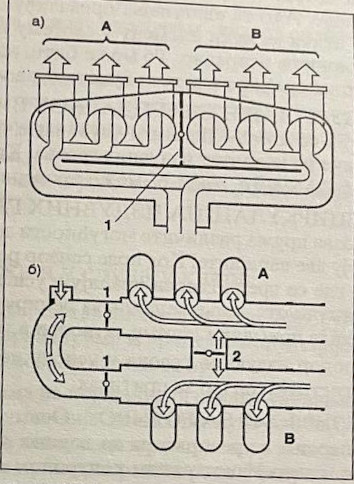
\includegraphics[height=4.8cm,keepaspectratio]{slike/15.2.jpg}
        \caption{Променљиви усисни системи са клапнама за прекопчавање дужине и резонанције усисног вода}
        \label{fig:usisni_vod}
    \end{minipage}
\end{figure}

%==================================================================
\section{Дијагностика (OBD), ECU и повезивање система (CAN)}
%==================================================================

\subsection{Дијагностичка функција система (OBD) и принудна вожња}

M-MOTRONIC поседује непрекидну самодијагностику која надзире протокомер,
изостанак паљења (преко равномерности обртања радилице), ефикасност
катализатора (поређењем сигнала предње и задње ламбда сонде), грејач сонде,
рециркулацију издувних гасова и заптивност резервоара (проба на пад притиска).
У случају квара неког сензора или излазног степена, ECU прелази у режим
\textbf{принудне вожње} користећи резервне параметре (нпр. при отказу паљења
на једном цилиндру искључује убризгавање у том цилиндру ради заштите катализатора).

\subsection{Електронска управљачка јединица (CPU)}

Управљачка јединица је смештена у чврсту металну кутију отпорну на температуре
од $-30^\circ\text{C}$ до $+60^\circ\text{C}$, влагу, вибрације и електромагнетне
сметње, са вишеполним прикључницама (35, 55 или 88 полова). Садржи улазна
заштитна кола, аналогно-дигиталне (AD) претвараче, микропроцесор, меморије
\textbf{EPROM/ROM} (програми и мапе података) и \textbf{RAM} (адаптивни подаци и
меморисане грешке, уз стално напајање са акумулатора), као и заштићене излазне
степене снаге (слика~\ref{fig:ecu_blok}).

\slikaV[0.75]{16.jpg}{Блок шема електронске управљачке јединице M-MOTRONIC система}{fig:ecu_blok}

\subsection{Повезивање са другим системима и CAN магистрала}

Уместо конвенционалног интерфејса где сваки сигнал захтева посебан проводник,
савремени системи (Motronic, аутоматски мењач GS, EGAS, ABS/ASR/MSR) повезују
се серијском магистралом података \textbf{CAN (Controller Area Network)} брзине
од $125\text{ kbit/s}$ до $1\text{ Mbit/s}$ (слика~\ref{fig:can_bus}).

\begin{kljucno}
\textbf{Карактеристике CAN система:}
\begin{itemize}[noitemsep]
    \item Линеарна \emph{Multi-Master} BUS структура (испад једне станице не омета рад осталих).
    \item Адресирање према садржају поруке (11-битни идентификатор поруке).
    \item Недеструктивно арбитрирање приоритета при истовременом слању.
    \item Кратак блок података (мање од 130 битова) за високу брзину одзива у реалном времену.
\end{itemize}
\end{kljucno}

\slika[0.65]{17.jpg}{Шематски приказ линеарне CAN BUS структуре}{fig:can_bus}


\end{document}
